
%(BEGIN_QUESTION)
% Copyright 2007, Tony R. Kuphaldt, released under the Creative Commons Attribution License (v 1.0)
% This means you may do almost anything with this work of mine, so long as you give me proper credit

{\it Limit switches} are often used on the doors of electrical enclosures and cabinets to automatically shut off power or shut down a machine's function if anyone opens the door for maintenance purposes.  The limit switch is typically mounted in such a way that a shut door holds the switch lever in the ``actuated'' position.  When the door opens wide, the limit switch lever is released and the switch returns to its ``normal'' status.

Draw the appropriate limit switch symbol in this ladder logic diagram so that the control circuit (shown as a rectangular box) gets shut down if ever someone opens the cabinet door:

$$\includegraphics[width=15.5cm]{i02967x01.eps}$$

Be sure to denote whether this limit switch needs to be normally-open (N.O.) or normally-closed (N.C.).

\underbar{file i02967}
%(END_QUESTION)





%(BEGIN_ANSWER)

$$\includegraphics[width=15.5cm]{i02967x02.eps}$$

%(END_ANSWER)





%(BEGIN_NOTES)

%INDEX% Switch, limit: mechanical actuation (direct contact)

%(END_NOTES)


